\problemname{\problemyamlname}

\begin{wrapfigure}{r}{5.5cm}
    \centering
    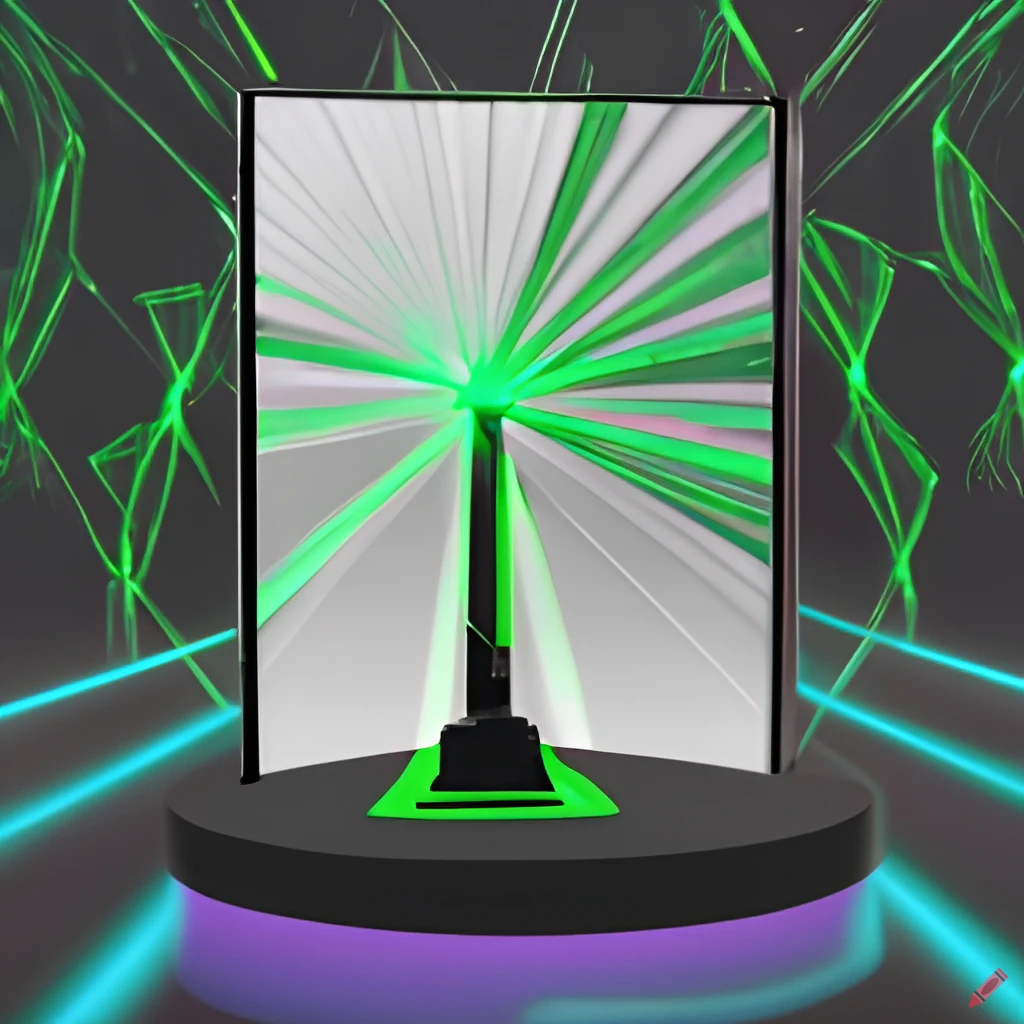
\includegraphics[width=5.5cm]{mirror.jpg}
\end{wrapfigure}

Finally, you're preparing to go to the annual KARWa-au-quai between UCLouvain and UMons, indispensable event in a student's life, where all vocations of singers are created, where all the big music labels come to pick out the future prodigies of tomorrow.

You need to be in the best of shapes, as much for your singing as for your appearance.
Nothing needs to be left to chance and you very much intend on impressing all of the sober people in the room\footnote{That means everyone, of course, this event is too important to drink before the end of the songs...} while you'll be on stage with your teammates to sing in choir.
On top of singing, you've prepared a little light show with mirrors to impress the whole crowd.

On stage, one of your teammates and yourself will be on the same line, facing the public.
Behind you, there's a large mirror parallel to this line.
You know the direct distance (perpendicular) between your position and the mirror, and you're going to activate the laser from your position to the mirror with a precise angle in relation with the perpendicular, in such a way that the laser beam bounces off of you teammate.

You must determine the distance your teammate must be so that they perfectly receive the laser beam.

\begin{figure}[h]
\centering
\begin{tikzpicture}[x=0.75pt,y=0.75pt,yscale=-1,xscale=1]
%Straight Lines [id:da9451307635096744]
\draw    (100.47,50.28) -- (501.47,50.78) ;
%Straight Lines [id:da37855877491674694]
\draw [color={rgb, 255:red, 0; green, 0; blue, 0 }  ,draw opacity=0.98 ] [dash pattern={on 0.75pt off 0.75pt}]  (292.97,49.9) .. controls (295.27,50.42) and (296.16,51.83) .. (295.63,54.13) .. controls (295.11,56.43) and (296,57.84) .. (298.3,58.36) .. controls (300.6,58.89) and (301.49,60.3) .. (300.96,62.6) .. controls (300.43,64.9) and (301.32,66.31) .. (303.62,66.83) .. controls (305.92,67.35) and (306.81,68.76) .. (306.29,71.06) .. controls (305.76,73.36) and (306.65,74.77) .. (308.95,75.29) .. controls (311.25,75.81) and (312.14,77.22) .. (311.62,79.52) .. controls (311.09,81.82) and (311.98,83.23) .. (314.28,83.75) .. controls (316.58,84.27) and (317.47,85.68) .. (316.94,87.98) .. controls (316.42,90.28) and (317.31,91.69) .. (319.61,92.21) .. controls (321.91,92.74) and (322.8,94.15) .. (322.27,96.45) .. controls (321.74,98.75) and (322.63,100.16) .. (324.93,100.68) .. controls (327.23,101.2) and (328.12,102.61) .. (327.6,104.91) .. controls (327.07,107.21) and (327.96,108.62) .. (330.26,109.14) .. controls (332.56,109.66) and (333.45,111.07) .. (332.93,113.37) .. controls (332.4,115.67) and (333.29,117.08) .. (335.59,117.6) .. controls (337.89,118.12) and (338.78,119.53) .. (338.25,121.83) .. controls (337.73,124.13) and (338.62,125.54) .. (340.92,126.07) .. controls (343.22,126.59) and (344.11,128) .. (343.58,130.3) .. controls (343.05,132.6) and (343.94,134.01) .. (346.24,134.53) .. controls (348.54,135.05) and (349.43,136.46) .. (348.91,138.76) .. controls (348.38,141.06) and (349.27,142.47) .. (351.57,142.99) .. controls (353.87,143.51) and (354.76,144.92) .. (354.24,147.22) .. controls (353.71,149.52) and (354.6,150.93) .. (356.9,151.45) .. controls (359.2,151.98) and (360.09,153.39) .. (359.56,155.69) .. controls (359.04,157.99) and (359.93,159.4) .. (362.23,159.92) .. controls (364.53,160.44) and (365.42,161.85) .. (364.89,164.15) .. controls (364.36,166.45) and (365.25,167.86) .. (367.55,168.38) .. controls (369.85,168.9) and (370.74,170.31) .. (370.22,172.61) .. controls (369.69,174.91) and (370.58,176.32) .. (372.88,176.84) .. controls (375.18,177.36) and (376.07,178.77) .. (375.55,181.07) .. controls (375.02,183.37) and (375.91,184.78) .. (378.21,185.3) .. controls (380.51,185.83) and (381.4,187.24) .. (380.87,189.54) .. controls (380.35,191.84) and (381.24,193.25) .. (383.54,193.77) .. controls (385.84,194.29) and (386.73,195.7) .. (386.2,198) .. controls (385.67,200.3) and (386.56,201.71) .. (388.86,202.23) .. controls (391.16,202.75) and (392.05,204.16) .. (391.53,206.46) .. controls (391,208.76) and (391.89,210.17) .. (394.19,210.69) .. controls (396.49,211.21) and (397.38,212.62) .. (396.86,214.92) .. controls (396.33,217.22) and (397.22,218.63) .. (399.52,219.16) .. controls (401.82,219.68) and (402.71,221.09) .. (402.18,223.39) .. controls (401.66,225.69) and (402.55,227.1) .. (404.85,227.62) -- (405.35,228.42) -- (406.95,230.96)(290.43,51.5) .. controls (292.73,52.02) and (293.62,53.43) .. (293.09,55.73) .. controls (292.57,58.03) and (293.46,59.44) .. (295.76,59.96) .. controls (298.06,60.48) and (298.95,61.89) .. (298.42,64.19) .. controls (297.9,66.49) and (298.79,67.9) .. (301.09,68.42) .. controls (303.39,68.95) and (304.28,70.36) .. (303.75,72.66) .. controls (303.22,74.96) and (304.11,76.37) .. (306.41,76.89) .. controls (308.71,77.41) and (309.6,78.82) .. (309.08,81.12) .. controls (308.55,83.42) and (309.44,84.83) .. (311.74,85.35) .. controls (314.04,85.87) and (314.93,87.28) .. (314.4,89.58) .. controls (313.88,91.88) and (314.77,93.29) .. (317.07,93.81) .. controls (319.37,94.33) and (320.26,95.74) .. (319.73,98.04) .. controls (319.21,100.34) and (320.1,101.75) .. (322.4,102.28) .. controls (324.7,102.8) and (325.59,104.21) .. (325.06,106.51) .. controls (324.53,108.81) and (325.42,110.22) .. (327.72,110.74) .. controls (330.02,111.26) and (330.91,112.67) .. (330.39,114.97) .. controls (329.86,117.27) and (330.75,118.68) .. (333.05,119.2) .. controls (335.35,119.72) and (336.24,121.13) .. (335.71,123.43) .. controls (335.19,125.73) and (336.08,127.14) .. (338.38,127.66) .. controls (340.68,128.19) and (341.57,129.6) .. (341.04,131.9) .. controls (340.52,134.2) and (341.41,135.61) .. (343.71,136.13) .. controls (346.01,136.65) and (346.9,138.06) .. (346.37,140.36) .. controls (345.84,142.66) and (346.73,144.07) .. (349.03,144.59) .. controls (351.33,145.11) and (352.22,146.52) .. (351.7,148.82) .. controls (351.17,151.12) and (352.06,152.53) .. (354.36,153.05) .. controls (356.66,153.57) and (357.55,154.98) .. (357.02,157.28) .. controls (356.5,159.58) and (357.39,160.99) .. (359.69,161.51) .. controls (361.99,162.04) and (362.88,163.45) .. (362.35,165.75) .. controls (361.83,168.05) and (362.72,169.46) .. (365.02,169.98) .. controls (367.32,170.5) and (368.21,171.91) .. (367.68,174.21) .. controls (367.15,176.51) and (368.04,177.92) .. (370.34,178.44) .. controls (372.64,178.96) and (373.53,180.37) .. (373.01,182.67) .. controls (372.48,184.97) and (373.37,186.38) .. (375.67,186.9) .. controls (377.97,187.42) and (378.86,188.83) .. (378.33,191.13) .. controls (377.81,193.43) and (378.7,194.84) .. (381,195.37) .. controls (383.3,195.89) and (384.19,197.3) .. (383.66,199.6) .. controls (383.14,201.9) and (384.03,203.31) .. (386.33,203.83) .. controls (388.63,204.35) and (389.52,205.76) .. (388.99,208.06) .. controls (388.46,210.36) and (389.35,211.77) .. (391.65,212.29) .. controls (393.95,212.81) and (394.84,214.22) .. (394.32,216.52) .. controls (393.79,218.82) and (394.68,220.23) .. (396.98,220.75) .. controls (399.28,221.28) and (400.17,222.69) .. (399.64,224.99) .. controls (399.12,227.29) and (400.01,228.7) .. (402.31,229.22) -- (402.81,230.02) -- (404.41,232.56) ;
\draw [shift={(410.47,239.38)}, rotate = 237.81] [fill={rgb, 255:red, 0; green, 0; blue, 0 }  ,fill opacity=0.98 ][line width=0.08]  [draw opacity=0] (10.72,-5.15) -- (0,0) -- (10.72,5.15) -- cycle    ;
%Curve Lines [id:da24698423041058837]
\draw    (168.97,208.38) .. controls (175.97,205.38) and (183.97,206.88) .. (186.47,212.88) ;
%Straight Lines [id:da4048989193409195]
\draw  [dash pattern={on 0.75pt off 0.75pt}]  (288.1,59.08) -- (286.48,61.61) .. controls (286.98,63.91) and (286.08,65.31) .. (283.78,65.82) .. controls (281.48,66.32) and (280.58,67.72) .. (281.08,70.02) .. controls (281.58,72.33) and (280.68,73.73) .. (278.37,74.23) .. controls (276.07,74.74) and (275.17,76.14) .. (275.67,78.44) .. controls (276.17,80.74) and (275.27,82.14) .. (272.97,82.64) .. controls (270.67,83.15) and (269.77,84.55) .. (270.27,86.85) .. controls (270.77,89.15) and (269.87,90.55) .. (267.57,91.06) .. controls (265.27,91.57) and (264.37,92.97) .. (264.87,95.27) .. controls (265.37,97.58) and (264.47,98.98) .. (262.16,99.47) .. controls (259.86,99.98) and (258.96,101.38) .. (259.46,103.68) .. controls (259.96,105.98) and (259.06,107.38) .. (256.76,107.89) .. controls (254.46,108.4) and (253.56,109.8) .. (254.06,112.1) .. controls (254.56,114.4) and (253.66,115.8) .. (251.36,116.3) .. controls (249.06,116.81) and (248.16,118.21) .. (248.66,120.51) .. controls (249.16,122.81) and (248.26,124.21) .. (245.96,124.72) .. controls (243.65,125.22) and (242.75,126.62) .. (243.25,128.93) .. controls (243.75,131.23) and (242.85,132.63) .. (240.55,133.13) .. controls (238.25,133.64) and (237.35,135.04) .. (237.85,137.34) .. controls (238.35,139.64) and (237.45,141.04) .. (235.15,141.55) .. controls (232.85,142.05) and (231.95,143.45) .. (232.45,145.75) .. controls (232.95,148.05) and (232.05,149.45) .. (229.75,149.96) .. controls (227.44,150.46) and (226.54,151.86) .. (227.04,154.17) .. controls (227.54,156.47) and (226.64,157.87) .. (224.34,158.38) .. controls (222.04,158.88) and (221.14,160.28) .. (221.64,162.58) .. controls (222.14,164.88) and (221.24,166.28) .. (218.94,166.79) .. controls (216.64,167.3) and (215.74,168.7) .. (216.24,171) .. controls (216.74,173.3) and (215.84,174.7) .. (213.54,175.21) .. controls (211.24,175.71) and (210.34,177.11) .. (210.84,179.41) .. controls (211.34,181.72) and (210.44,183.12) .. (208.13,183.62) .. controls (205.83,184.13) and (204.93,185.53) .. (205.43,187.83) .. controls (205.93,190.13) and (205.03,191.53) .. (202.73,192.04) .. controls (200.43,192.54) and (199.53,193.94) .. (200.03,196.24) .. controls (200.53,198.54) and (199.63,199.94) .. (197.33,200.45) .. controls (195.03,200.96) and (194.13,202.36) .. (194.63,204.66) .. controls (195.13,206.97) and (194.23,208.37) .. (191.92,208.86) .. controls (189.62,209.37) and (188.72,210.77) .. (189.22,213.07) .. controls (189.72,215.37) and (188.82,216.77) .. (186.52,217.28) .. controls (184.22,217.79) and (183.32,219.19) .. (183.82,221.49) .. controls (184.32,223.79) and (183.42,225.19) .. (181.12,225.69) .. controls (178.82,226.2) and (177.92,227.6) .. (178.42,229.9) .. controls (178.92,232.21) and (178.02,233.61) .. (175.71,234.11) .. controls (173.41,234.62) and (172.51,236.02) .. (173.01,238.32) -- (170.96,241.51) -- (170.96,241.51)(285.58,57.46) -- (283.95,59.99) .. controls (284.45,62.29) and (283.55,63.69) .. (281.25,64.19) .. controls (278.95,64.7) and (278.05,66.1) .. (278.55,68.4) .. controls (279.05,70.7) and (278.15,72.1) .. (275.85,72.61) .. controls (273.55,73.12) and (272.65,74.52) .. (273.15,76.82) .. controls (273.65,79.12) and (272.75,80.52) .. (270.45,81.02) .. controls (268.14,81.52) and (267.24,82.92) .. (267.74,85.23) .. controls (268.24,87.53) and (267.34,88.93) .. (265.04,89.44) .. controls (262.74,89.95) and (261.84,91.35) .. (262.34,93.65) .. controls (262.84,95.95) and (261.94,97.35) .. (259.64,97.85) .. controls (257.34,98.36) and (256.44,99.76) .. (256.94,102.06) .. controls (257.44,104.36) and (256.54,105.76) .. (254.24,106.27) .. controls (251.94,106.78) and (251.04,108.18) .. (251.54,110.48) .. controls (252.04,112.79) and (251.14,114.19) .. (248.83,114.68) .. controls (246.53,115.19) and (245.63,116.59) .. (246.13,118.89) .. controls (246.63,121.19) and (245.73,122.59) .. (243.43,123.1) .. controls (241.13,123.6) and (240.23,125) .. (240.73,127.3) .. controls (241.23,129.6) and (240.33,131) .. (238.03,131.51) .. controls (235.73,132.02) and (234.83,133.42) .. (235.33,135.72) .. controls (235.83,138.03) and (234.93,139.43) .. (232.62,139.93) .. controls (230.32,140.43) and (229.42,141.83) .. (229.92,144.13) .. controls (230.42,146.43) and (229.52,147.83) .. (227.22,148.34) .. controls (224.92,148.85) and (224.02,150.25) .. (224.52,152.55) .. controls (225.02,154.85) and (224.12,156.25) .. (221.82,156.76) .. controls (219.52,157.26) and (218.62,158.66) .. (219.12,160.96) .. controls (219.62,163.26) and (218.72,164.66) .. (216.42,165.17) .. controls (214.11,165.67) and (213.21,167.07) .. (213.71,169.38) .. controls (214.21,171.68) and (213.31,173.08) .. (211.01,173.59) .. controls (208.71,174.09) and (207.81,175.49) .. (208.31,177.79) .. controls (208.81,180.09) and (207.91,181.49) .. (205.61,182) .. controls (203.31,182.51) and (202.41,183.91) .. (202.91,186.21) .. controls (203.41,188.51) and (202.51,189.91) .. (200.21,190.41) .. controls (197.9,190.91) and (197,192.31) .. (197.5,194.62) .. controls (198,196.92) and (197.1,198.32) .. (194.8,198.83) .. controls (192.5,199.34) and (191.6,200.74) .. (192.1,203.04) .. controls (192.6,205.34) and (191.7,206.74) .. (189.4,207.24) .. controls (187.1,207.75) and (186.2,209.15) .. (186.7,211.45) .. controls (187.2,213.75) and (186.3,215.15) .. (184,215.66) .. controls (181.7,216.17) and (180.8,217.57) .. (181.3,219.87) .. controls (181.8,222.18) and (180.9,223.58) .. (178.59,224.07) .. controls (176.29,224.58) and (175.39,225.98) .. (175.89,228.28) .. controls (176.39,230.58) and (175.49,231.98) .. (173.19,232.49) .. controls (170.89,233) and (169.99,234.4) .. (170.49,236.7) -- (168.44,239.89) -- (168.44,239.89) ;
\draw [shift={(291.7,50.7)}, rotate = 122.7] [fill={rgb, 255:red, 0; green, 0; blue, 0 }  ][line width=0.08]  [draw opacity=0] (8.93,-4.29) -- (0,0) -- (8.93,4.29) -- cycle    ;
%Straight Lines [id:da7530300672363276]
\draw  [dash pattern={on 4.5pt off 4.5pt}]  (170.48,50.7) -- (169.7,240.7) ;

% Text Node
\draw (175.98,190.17) node [anchor=north west][inner sep=0.75pt]   [align=left] {$\displaystyle \alpha $};
% Text Node
\draw (170.68,113.27) node [anchor=north west][inner sep=0.75pt]   [align=left] {$\displaystyle d$};
% Text Node
\draw (150.68,239.27) node [anchor=north west][inner sep=0.75pt]   [align=left] {You};
% Text Node
\draw (375.68,240.77) node [anchor=north west][inner sep=0.75pt]   [align=left] {Teammate};
% Text Node
\draw (270.18,27.27) node [anchor=north west][inner sep=0.75pt]   [align=left] {Mirror};
\end{tikzpicture}
\end{figure}



\begin{Input}
	The input consists of :
	\begin{itemize}
		\item One line with an integer $d$ ($0 < d \le 10^6$), the distance which separates you with the mirror.
		\item One line with an integer $\alpha$ ($0 < \alpha < 90$), the angle in degrees of your laser in relation with the perpendicular towards the mirror.
	\end{itemize}
\end{Input}

\begin{Output}
	The distance between your teammate and yourself so that they receive the laser beam on themselves.
	The answer must have an absolute or relative error of maximum $10^{-6}$.
\end{Output}
